% Options for packages loaded elsewhere
\PassOptionsToPackage{unicode}{hyperref}
\PassOptionsToPackage{hyphens}{url}
%
\documentclass[
  10pt,
]{article}
\usepackage{amsmath,amssymb}
\usepackage{iftex}
\ifPDFTeX
  \usepackage[T1]{fontenc}
  \usepackage[utf8]{inputenc}
  \usepackage{textcomp} % provide euro and other symbols
\else % if luatex or xetex
  \usepackage{unicode-math} % this also loads fontspec
  \defaultfontfeatures{Scale=MatchLowercase}
  \defaultfontfeatures[\rmfamily]{Ligatures=TeX,Scale=1}
\fi
\usepackage{lmodern}
\ifPDFTeX\else
  % xetex/luatex font selection
\fi
% Use upquote if available, for straight quotes in verbatim environments
\IfFileExists{upquote.sty}{\usepackage{upquote}}{}
\IfFileExists{microtype.sty}{% use microtype if available
  \usepackage[]{microtype}
  \UseMicrotypeSet[protrusion]{basicmath} % disable protrusion for tt fonts
}{}
\makeatletter
\@ifundefined{KOMAClassName}{% if non-KOMA class
  \IfFileExists{parskip.sty}{%
    \usepackage{parskip}
  }{% else
    \setlength{\parindent}{0pt}
    \setlength{\parskip}{6pt plus 2pt minus 1pt}}
}{% if KOMA class
  \KOMAoptions{parskip=half}}
\makeatother
\usepackage{xcolor}
\usepackage{color}
\usepackage{fancyvrb}
\newcommand{\VerbBar}{|}
\newcommand{\VERB}{\Verb[commandchars=\\\{\}]}
\DefineVerbatimEnvironment{Highlighting}{Verbatim}{commandchars=\\\{\}}
% Add ',fontsize=\small' for more characters per line
\newenvironment{Shaded}{}{}
\newcommand{\AlertTok}[1]{\textcolor[rgb]{1.00,0.00,0.00}{\textbf{#1}}}
\newcommand{\AnnotationTok}[1]{\textcolor[rgb]{0.38,0.63,0.69}{\textbf{\textit{#1}}}}
\newcommand{\AttributeTok}[1]{\textcolor[rgb]{0.49,0.56,0.16}{#1}}
\newcommand{\BaseNTok}[1]{\textcolor[rgb]{0.25,0.63,0.44}{#1}}
\newcommand{\BuiltInTok}[1]{\textcolor[rgb]{0.00,0.50,0.00}{#1}}
\newcommand{\CharTok}[1]{\textcolor[rgb]{0.25,0.44,0.63}{#1}}
\newcommand{\CommentTok}[1]{\textcolor[rgb]{0.38,0.63,0.69}{\textit{#1}}}
\newcommand{\CommentVarTok}[1]{\textcolor[rgb]{0.38,0.63,0.69}{\textbf{\textit{#1}}}}
\newcommand{\ConstantTok}[1]{\textcolor[rgb]{0.53,0.00,0.00}{#1}}
\newcommand{\ControlFlowTok}[1]{\textcolor[rgb]{0.00,0.44,0.13}{\textbf{#1}}}
\newcommand{\DataTypeTok}[1]{\textcolor[rgb]{0.56,0.13,0.00}{#1}}
\newcommand{\DecValTok}[1]{\textcolor[rgb]{0.25,0.63,0.44}{#1}}
\newcommand{\DocumentationTok}[1]{\textcolor[rgb]{0.73,0.13,0.13}{\textit{#1}}}
\newcommand{\ErrorTok}[1]{\textcolor[rgb]{1.00,0.00,0.00}{\textbf{#1}}}
\newcommand{\ExtensionTok}[1]{#1}
\newcommand{\FloatTok}[1]{\textcolor[rgb]{0.25,0.63,0.44}{#1}}
\newcommand{\FunctionTok}[1]{\textcolor[rgb]{0.02,0.16,0.49}{#1}}
\newcommand{\ImportTok}[1]{\textcolor[rgb]{0.00,0.50,0.00}{\textbf{#1}}}
\newcommand{\InformationTok}[1]{\textcolor[rgb]{0.38,0.63,0.69}{\textbf{\textit{#1}}}}
\newcommand{\KeywordTok}[1]{\textcolor[rgb]{0.00,0.44,0.13}{\textbf{#1}}}
\newcommand{\NormalTok}[1]{#1}
\newcommand{\OperatorTok}[1]{\textcolor[rgb]{0.40,0.40,0.40}{#1}}
\newcommand{\OtherTok}[1]{\textcolor[rgb]{0.00,0.44,0.13}{#1}}
\newcommand{\PreprocessorTok}[1]{\textcolor[rgb]{0.74,0.48,0.00}{#1}}
\newcommand{\RegionMarkerTok}[1]{#1}
\newcommand{\SpecialCharTok}[1]{\textcolor[rgb]{0.25,0.44,0.63}{#1}}
\newcommand{\SpecialStringTok}[1]{\textcolor[rgb]{0.73,0.40,0.53}{#1}}
\newcommand{\StringTok}[1]{\textcolor[rgb]{0.25,0.44,0.63}{#1}}
\newcommand{\VariableTok}[1]{\textcolor[rgb]{0.10,0.09,0.49}{#1}}
\newcommand{\VerbatimStringTok}[1]{\textcolor[rgb]{0.25,0.44,0.63}{#1}}
\newcommand{\WarningTok}[1]{\textcolor[rgb]{0.38,0.63,0.69}{\textbf{\textit{#1}}}}
\usepackage{longtable,booktabs,array}
\usepackage{calc} % for calculating minipage widths
% Correct order of tables after \paragraph or \subparagraph
\usepackage{etoolbox}
\makeatletter
\patchcmd\longtable{\par}{\if@noskipsec\mbox{}\fi\par}{}{}
\makeatother
% Allow footnotes in longtable head/foot
\IfFileExists{footnotehyper.sty}{\usepackage{footnotehyper}}{\usepackage{footnote}}
\makesavenoteenv{longtable}
\usepackage{graphicx}
\makeatletter
\def\maxwidth{\ifdim\Gin@nat@width>\linewidth\linewidth\else\Gin@nat@width\fi}
\def\maxheight{\ifdim\Gin@nat@height>\textheight\textheight\else\Gin@nat@height\fi}
\makeatother
% Scale images if necessary, so that they will not overflow the page
% margins by default, and it is still possible to overwrite the defaults
% using explicit options in \includegraphics[width, height, ...]{}
\setkeys{Gin}{width=\maxwidth,height=\maxheight,keepaspectratio}
% Set default figure placement to htbp
\makeatletter
\def\fps@figure{htbp}
\makeatother
\setlength{\emergencystretch}{3em} % prevent overfull lines
\providecommand{\tightlist}{%
  \setlength{\itemsep}{0pt}\setlength{\parskip}{0pt}}
\setcounter{secnumdepth}{-\maxdimen} % remove section numbering
\newlength{\cslhangindent}
\setlength{\cslhangindent}{1.5em}
\newlength{\csllabelwidth}
\setlength{\csllabelwidth}{3em}
\newlength{\cslentryspacingunit} % times entry-spacing
\setlength{\cslentryspacingunit}{\parskip}
\newenvironment{CSLReferences}[2] % #1 hanging-ident, #2 entry spacing
 {% don't indent paragraphs
  \setlength{\parindent}{0pt}
  % turn on hanging indent if param 1 is 1
  \ifodd #1
  \let\oldpar\par
  \def\par{\hangindent=\cslhangindent\oldpar}
  \fi
  % set entry spacing
  \setlength{\parskip}{#2\cslentryspacingunit}
 }%
 {}
\usepackage{calc}
\newcommand{\CSLBlock}[1]{#1\hfill\break}
\newcommand{\CSLLeftMargin}[1]{\parbox[t]{\csllabelwidth}{#1}}
\newcommand{\CSLRightInline}[1]{\parbox[t]{\linewidth - \csllabelwidth}{#1}\break}
\newcommand{\CSLIndent}[1]{\hspace{\cslhangindent}#1}
\ifLuaTeX
\usepackage[bidi=basic]{babel}
\else
\usepackage[bidi=default]{babel}
\fi
\babelprovide[main,import]{american}
% get rid of language-specific shorthands (see #6817):
\let\LanguageShortHands\languageshorthands
\def\languageshorthands#1{}
% SPDX-License-Identifier: Apache-2.0
\usepackage[letterpaper,margin=0.82in,headheight=15pt,headsep=19pt,footskip=28pt]{geometry}
\usepackage{fontspec}
\setmainfont{DejaVu Serif}
\setsansfont{DejaVu Sans}
\setmonofont[Scale=0.82]{DejaVu Sans Mono}
\usepackage{microtype,amsmath,amssymb,booktabs,longtable,array,graphicx,xcolor}
\usepackage{fancyhdr,titlesec,enumitem,caption,needspace,etoolbox,tcolorbox}
\definecolor{DeepPurple}{HTML}{301356}
\definecolor{RoyalPurple}{HTML}{6C39B7}
\definecolor{PalePurple}{HTML}{F3EDF9}
\definecolor{Ink}{HTML}{231B33}
\definecolor{Muted}{HTML}{61566E}
\color{Ink}
\setlength{\parindent}{0pt}
\setlength{\parskip}{5pt plus1pt}
\setlength{\emergencystretch}{3em}
\linespread{1.035}
\pagestyle{fancy}\fancyhf{}
\fancyhead[L]{\footnotesize\sffamily\color{DeepPurple}AGI ALPHA FLYWHEEL}
\fancyhead[R]{\footnotesize\sffamily DIGITAL / R1}
\fancyfoot[L]{\scriptsize\sffamily MONTREAL.AI | Research review edition}
\fancyfoot[R]{\small\sffamily\thepage}
\renewcommand{\headrulewidth}{0.35pt}
\titleformat{\section}{\LARGE\sffamily\bfseries\color{DeepPurple}}{\thesection}{0.7em}{}
\titleformat{\subsection}{\large\sffamily\bfseries\color{DeepPurple}}{\thesubsection}{0.6em}{}
\titleformat{\subsubsection}{\normalsize\sffamily\bfseries\color{DeepPurple}}{\thesubsubsection}{0.5em}{}
\titlespacing*{\section}{0pt}{1.2em}{0.5em}
\titlespacing*{\subsection}{0pt}{0.8em}{0.3em}
\pretocmd{\subsection}{\Needspace{8\baselineskip}}{}{}
\setlist{nosep,leftmargin=1.4em,topsep=4pt,itemsep=2pt}
\captionsetup{font=small,labelfont={bf,sf},textfont=sf}
\setlength{\tabcolsep}{5pt}\renewcommand{\arraystretch}{1.18}
\AtBeginEnvironment{longtable}{\small}
\BeforeBeginEnvironment{longtable}{\Needspace{5\baselineskip}}
\newcommand{\editionbreak}{\par\bigskip\Needspace{8\baselineskip}}
\newcommand{\resultbox}[1]{\begin{tcolorbox}[colback=PalePurple,colframe=DeepPurple,boxrule=0pt,leftrule=3pt,arc=0pt,left=10pt,right=10pt,top=8pt,bottom=8pt]#1\end{tcolorbox}}
\AtBeginDocument{\hypersetup{colorlinks=true,linkcolor=DeepPurple,citecolor=DeepPurple,urlcolor=RoyalPurple,pdfauthor={Vincent Boucher},pdftitle={AGI ALPHA FLYWHEEL - When Capability Creates Opportunity},pdfsubject={From a numerical failure to a verified digital answer}}}
\ifLuaTeX
  \usepackage{selnolig}  % disable illegal ligatures
\fi
\IfFileExists{bookmark.sty}{\usepackage{bookmark}}{\usepackage{hyperref}}
\IfFileExists{xurl.sty}{\usepackage{xurl}}{} % add URL line breaks if available
\urlstyle{same}
\hypersetup{
  pdflang={en-US},
  hidelinks,
  pdfcreator={LaTeX via pandoc}}

\usepackage{etoolbox}
\makeatletter
\providecommand{\subtitle}[1]{% add subtitle to \maketitle
  \apptocmd{\@title}{\par {\large #1 \par}}{}{}
}
\makeatother
\subtitle{From a numerical failure to a verified digital answer}
\author{}
\date{}

\begin{document}

% SPDX-License-Identifier: Apache-2.0
\begin{titlepage}
\pagecolor{DeepPurple}\color{white}
\vspace*{0.45in}
{\sffamily\small MONTREAL.AI\hfill DIGITAL-20261027-R1\par}
\vspace{0.85in}
{\sffamily\fontsize{35}{40}\selectfont\bfseries AGI ALPHA\\FLYWHEEL\par}
\vspace{0.24in}
{\sffamily\fontsize{23}{29}\selectfont When Capability\\Creates Opportunity\par}
\vspace{0.42in}
{\color{white!70}\rule{0.9\linewidth}{0.7pt}\par}
\vspace{0.25in}
{\sffamily\fontsize{18}{24}\selectfont From a numerical failure\\to a verified digital answer\par}
\vspace{0.25in}
{\large Transformational Intelligence, Experience-Trained Specialists and the Expanding Frontier of Profitable Work\par}
\vfill
{\sffamily\small FIND YOUR ALPHA. BUILD YOUR SUCCESSOR $\Omega$.\par}\vspace{0.25in}
{\sffamily\bfseries Vincent Boucher\par}
{\sffamily President of MONTREAL.AI\par}
\vspace{0.3in}
{\sffamily\small 27 October 2026 | Research review edition\par}
\vspace{0.2in}
{\small Three live agent workflows. One public numerical mission.\\64 fresh checks per workflow. Three complete passes.\par}
\vspace{0.15in}
{\footnotesize Useful digital construction established within the frozen scope. General Operational Alpha, novel numerical capability and realized commercial return are not established.\par}
\end{titlepage}
\nopagecolor\color{Ink}\setcounter{page}{1}

\hypertarget{a-useful-answer-with-its-limits-attached}{%
\section{A useful answer, with its limits
attached}\label{a-useful-answer-with-its-limits-attached}}

\textbf{A public numerical failure can now be turned into an
inspectable, executable answer within a bounded agent mission.} This
edition delivers a scalar beta-quantile compatibility kernel, a
command-line interface, three frozen implementations, independent
numerical checks, a complete replay package and an explicit commercial
decision. It changes what a scientific software team can do immediately:
reproduce an extreme-tail failure, obtain a checked replacement value
within a stated domain, and inspect the evidence before deciding whether
to integrate the component.

The concrete example matters. For probability \(10^{-16}\) and beta
shape parameters \(a=0.5\), \(b=3\), the installed SciPy 1.17.0
environment returned a quantile of \textbf{0.5}. The independently
evaluated value is approximately
\textbf{\(2.844444444444444\times10^{-33}\)}. The public report supplied
the failure and a candidate numerical recipe. We did not discover that
formulation. We converted it into bounded, failure-aware artifacts and
tested the contribution of different ways of operating the available
assistant. (\protect\hyperlink{ref-scipyissue}{chrisb83 2026})

All three workflows passed the \textbf{64 fresh confirmation checks}: 56
numerical or endpoint cases and eight required refusals. Ordinary
competent operation and expert operation also handled a separately
disclosed, already-known subnormal rounding trap; the original
conventional implementation failed that diagnostic. Its correction is
preserved separately. The fresh bank is one mission's case bank, not 64
independent missions or customers.

\begin{quote}
\textbf{Decision: retain and deliver the useful engineering; pursue only
a customer-funded qualification pilot. Do not promote this edition as an
exclusive numerical breakthrough, a measured general Operational Alpha
advantage, or a realized profitable business.}
\end{quote}

\hypertarget{three-verdicts}{%
\subsection{Three verdicts}\label{three-verdicts}}

\begin{longtable}[]{@{}
  >{\raggedright\arraybackslash}p{(\columnwidth - 4\tabcolsep) * \real{0.3333}}
  >{\raggedright\arraybackslash}p{(\columnwidth - 4\tabcolsep) * \real{0.3333}}
  >{\raggedright\arraybackslash}p{(\columnwidth - 4\tabcolsep) * \real{0.3333}}@{}}
\toprule\noalign{}
\begin{minipage}[b]{\linewidth}\raggedright
Question
\end{minipage} & \begin{minipage}[b]{\linewidth}\raggedright
What this edition establishes
\end{minipage} & \begin{minipage}[b]{\linewidth}\raggedright
What remains missing
\end{minipage} \\
\midrule\noalign{}
\endhead
\bottomrule\noalign{}
\endlastfoot
Commercial delivery & An executable digital artifact accepted by the
frozen research contract; a conditional service model with explicit
thresholds & External buyer acceptance, willingness to pay, commitments,
collections and complete actual costs \\
Operational Alpha & Live, tool-using implementations by ordinary and
expert agents; both pass the fresh bank and the rounding diagnostic & A
demonstrated improvement in accepted quality or complete economics from
expert operation \\
Transformational contribution & A useful bridge from a reported failure
to a bounded executable outcome & New numerical capability beyond the
strongest identified established methods; an independent discovery
comparison \\
\end{longtable}

The program's ambition remains larger than this result. Its discipline
is to preserve a useful construction without borrowing an achievement
from a failed hypothesis. The most productive successor may begin with a
reliable piece of engineering and a sharper question, rather than with a
claim of superiority.

The work was AI-assisted under the requested authorship. External
authors retain credit for the report, recipe, libraries and foundational
methods. No external peer review, production adoption or paid customer
approval is implied.

\clearpage

\hypertarget{the-opportunity-and-the-early-challenge}{%
\section{The opportunity and the early
challenge}\label{the-opportunity-and-the-early-challenge}}

\hypertarget{who-benefits-and-what-changes}{%
\subsection{Who benefits, and what
changes}\label{who-benefits-and-what-changes}}

The immediate beneficiary is a maintainer or scientific software team
evaluating a beta-tail calculation. Such a recipient needs more than a
plausible formula: a reproducible failure, a bounded replacement,
evidence for extreme and invalid inputs, and clear integration limits.
Wrong finite values are particularly troublesome because a program may
continue without an exception. Several observed failures emitted
warnings; an application that ignores them can still consume an
incorrect finite value. Whether a particular recipient's downstream
decision is materially affected remains a customer-specific question;
this study does not invent a deployed failure or financial loss.

The useful opportunity is \textbf{rapid numerical incident
qualification}: assembling a precise failure report and a tested
compatibility component from public inputs before an upstream release or
a local migration is available. The changes making this operationally
plausible are accessible source and issue histories, current numerical
libraries, arbitrary-precision arithmetic and an assistant capable of
reading code, compiling kernels, diagnosing failed checks and packaging
evidence. This study observes that combination working locally. It does
not establish that organizations were previously incapable of doing the
same work.

Our shortlist was concentrated in scientific software, not a claim to an
exhaustive cross-industry search. The preceding gap sprint had already
explored broader opportunities. We narrowed the continuation to
deliverable public incidents where the reasoning and execution were real
and physical fabrication was unnecessary.

\begin{longtable}[]{@{}
  >{\raggedright\arraybackslash}p{(\columnwidth - 4\tabcolsep) * \real{0.3333}}
  >{\raggedright\arraybackslash}p{(\columnwidth - 4\tabcolsep) * \real{0.3333}}
  >{\raggedright\arraybackslash}p{(\columnwidth - 4\tabcolsep) * \real{0.3333}}@{}}
\toprule\noalign{}
\begin{minipage}[b]{\linewidth}\raggedright
Candidate
\end{minipage} & \begin{minipage}[b]{\linewidth}\raggedright
Unmet outcome and beneficiary
\end{minipage} & \begin{minipage}[b]{\linewidth}\raggedright
Strongest early alternative and disposition
\end{minipage} \\
\midrule\noalign{}
\endhead
\bottomrule\noalign{}
\endlastfoot
Beta-tail failure qualification & Checked scalar answers and an
inspectable compatibility kernel for a numerical software team & Current
Boost.Math plus ordinary high-precision methods solved the public
examples. Selected for delivery and agent comparison; algorithmic
novelty rejected early. \\
Boundary confidence intervals & Reliable boundary behavior and a
validated repair for statistical software users & Existing active repair
PRs already owned the relevant statsmodels issues. Excluded rather than
duplicate ongoing work. \\
Kronecker-product correctness & A usable symbolic correction and
regression evidence for SymPy users & An active repair PR already
addressed the report. Excluded from construction. \\
\end{longtable}

The exact issue and PR records, rejected candidates and initial search
notes are included in the evidence package. Statsmodels issues
10536/10538 had active PRs 10537/10539; SymPy issue 30860 had active PR
30863 at inspection. (\protect\hyperlink{ref-statsmodels}{statsmodels
contributors 2026}; \protect\hyperlink{ref-sympy}{SymPy contributors
2026})

\hypertarget{conventional-falsification-came-first}{%
\subsection{Conventional falsification came
first}\label{conventional-falsification-came-first}}

Before the three agent constructions began, a separate workstream
compiled current Boost.Math at commit
\texttt{70a36632cfbfe6a862cd8a5b88b357ca3a770a3d}. A double-precision
policy disabling promotion, with safe error handling and 400 root
iterations, solved \textbf{all five public examples}. Its maximum
relative error against the 80-digit public-recipe reference was
approximately \(2.008\times10^{-14}\). Raising the cap to 2,000 did not
change that five-case result. A long-double configuration failed one
example at both caps; the failed configuration remains in the record.

This is a meaningful established alternative. SciPy itself documents
that \texttt{betaincinv} wraps Boost's \texttt{ibeta\_inv}; the Boost
interface already exposes precision and error policies. A successful
current-Boost configuration is therefore not an invented numerical
method. (\protect\hyperlink{ref-scipydocs}{SciPy Developers 2026};
\protect\hyperlink{ref-boost}{Boost.Math Developers 2026})

\textbf{Selection changed because of this evidence.} The candidate
survived as a useful digital delivery and an operational comparison. Its
exclusive technical-breakthrough claim did not survive. Public-source
formulation credit stays with the reporter; execution comparators
received that formulation in full.

\editionbreak

\hypertarget{what-was-actually-compared}{%
\section{What was actually compared}\label{what-was-actually-compared}}

\hypertarget{equivalent-information-capable-baselines}{%
\subsection{Equivalent information, capable
baselines}\label{equivalent-information-capable-baselines}}

Three new agent workstreams received the same common prompt, public
report and proposed recipe, pinned source extracts,
conventional-challenge results, libraries, acceptance contract, tool
access and resource limits. Each could inspect source, write code,
compile a C++ kernel, run tests and recover from failures. Ordinary
competent use was not reduced to a single prompt or forbidden from
verification.

The expert arm received an explicit operating checklist: extract
obligations, plan numerical regimes, verify independently, preserve
failures and recover before freezing. The conventional arm was asked to
compose the strongest practical established numerical techniques. Its
implementation was built by an assistant too; it is \textbf{not a
measured human-team trial}. The distinction is workflow and instruction,
not a claim that conventional reasoning excludes tool-using AI.

All arms used the inherited available assistant configuration. The
environment supplied the label \textbf{GPT-6 Astra Pro}.
Provider-attested backend identity, temperature, sampling seed, token
counts and billed cost were not exposed. These fields are recorded as
unknown. No independent API endpoint was invoked to manufacture a
stronger identity claim. The model work and local execution were live;
this was not a simulation of successful model behavior. The result is
narrower than a fully controlled, provider-metered same-model trial.

Computer execution consisted of shell commands, source inspection,
compilation, numerical tests and file construction. No graphical
interface performance was measured. No live \texttt{*.agent.agi.eth}
identity, external settlement or production authority was asserted.

\hypertarget{a-bounded-construction-budget}{%
\subsection{A bounded construction
budget}\label{a-bounded-construction-budget}}

The continuation reserved 120 minutes, starting at 18:06:05 on 27
October 2026 in Montréal, using existing authorized resources.
Opportunity selection and conventional falsification preceded
construction. Each implementation received a 15-minute, 25-tool
construction ceiling with no subagents. The remaining continuation
budget covered fresh confirmation, independent checking, economics,
reproducible delivery and publication preparation.

\begin{figure}
\centering
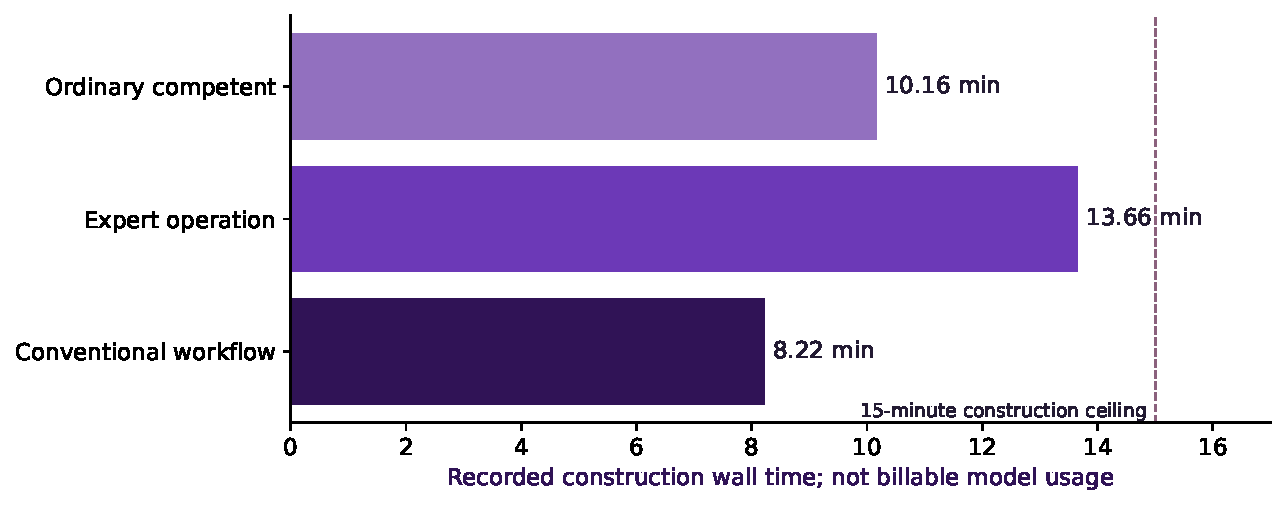
\includegraphics{figures/construction_time.pdf}
\caption{Recorded construction time. Expert operation took longer in
this single trial. This is elapsed construction time, not token usage,
billable cost or a population estimate.}
\end{figure}

\begin{longtable}[]{@{}
  >{\raggedright\arraybackslash}p{(\columnwidth - 6\tabcolsep) * \real{0.2500}}
  >{\raggedleft\arraybackslash}p{(\columnwidth - 6\tabcolsep) * \real{0.2500}}
  >{\raggedright\arraybackslash}p{(\columnwidth - 6\tabcolsep) * \real{0.2500}}
  >{\raggedleft\arraybackslash}p{(\columnwidth - 6\tabcolsep) * \real{0.2500}}@{}}
\toprule\noalign{}
\begin{minipage}[b]{\linewidth}\raggedright
Arm
\end{minipage} & \begin{minipage}[b]{\linewidth}\raggedleft
Recorded construction time
\end{minipage} & \begin{minipage}[b]{\linewidth}\raggedright
Source freeze, UTC
\end{minipage} & \begin{minipage}[b]{\linewidth}\raggedleft
Tool count as recorded
\end{minipage} \\
\midrule\noalign{}
\endhead
\bottomrule\noalign{}
\endlastfoot
Ordinary competent & 10.16 min & 22:32:41 & 21 \\
Expert operation & 13.66 min & 22:36:25 & 23 \\
Conventional workflow & 8.22 min & 22:30:53 & 13 \\
\end{longtable}

Tool-count conventions differ: the expert manifest includes progress
messages, while the conventional count describes execution calls. They
are traceability records, not a normalized efficiency measure. Timings
start at the first recorded agent timestamp, not a provider scheduling
boundary. The expert also recovered from a task-storage exhaustion
during packaging; numerical work and original failed packaging evidence
were preserved.

\hypertarget{discovery-and-execution-are-separate-experiments}{%
\subsection{Discovery and execution are separate
experiments}\label{discovery-and-execution-are-separate-experiments}}

No discovery advantage is claimed. The user supplied the program's
objective; the continuation search found the public issue; the issue
supplied the mathematical recipe. Every execution arm received it. A
future discovery comparison would need equivalent initial information
before revealing that recipe and a prespecified way to score the
usefulness and originality of the formulation. A technical tie cannot
supply that missing experiment retrospectively.

\editionbreak

\hypertarget{the-accepted-digital-contract}{%
\section{The accepted digital
contract}\label{the-accepted-digital-contract}}

The delivered object is deliberately bounded: \textbf{a scalar
compatibility component}, not a drop-in replacement for all SciPy
distributions, array broadcasting, accelerators, automatic
differentiation or every positive beta shape.

A request contains an identifier and three numbers: probability \(q\)
and shapes \(a,b\). The interpretation is the exact binary64 value
received by Python. The accepted numerical domain is

\[
0\le q\le1,\qquad 0.25\le a,b\le10^6,\qquad \min(a,b)\le100.
\]

The result preserves the identifier and returns a status with a value or
a refusal. Exact probabilities zero and one require their corresponding
endpoint values. An interior true quantile that rounds to binary64 zero
requires an explicit \texttt{underflow} status. Unsupported positive
shapes are distinguished from invalid inputs. Booleans, strings,
nonfinite values, nonpositive shapes and out-of-range probabilities are
not silently coerced into numerical success.

For a verified reference value \(r\) strictly between zero and one, the
frozen acceptance tolerance is

\[
|\widehat x-r|\le \max\{2\,\operatorname{ulp}(r),\;10^{-11}\min(r,1-r)\}.
\]

A representable positive reference may not be replaced with zero.
Correct endpoint, underflow and refusal behavior is checked explicitly.
A computation that cannot establish an answer returns \texttt{failed}; a
plausible finite number does not automatically count as success.

\hypertarget{how-the-construction-works}{%
\subsection{How the construction
works}\label{how-the-construction-works}}

The three implementations combine established instruments: a pinned
Boost inverse, analytic special cases, incomplete-beta continued
fractions, symmetry, log-domain arithmetic and high-precision
safeguarded inversion when needed. This composition protects against
numerical scale and unsupported inputs. Its scientific ingredients are
conventional. Definitions, symmetry, the integer-shape binomial identity
and continued fractions appear in NIST's reference treatment.
(\protect\hyperlink{ref-dlmf}{National Institute of Standards and
Technology 2026})

The ordinary implementation is the recommended research entry point
because it passed the primary contract and the disclosed rounding
regression with less recorded construction time than the expert arm.
That is a local delivery choice, not a universal ranking. All original
implementations remain available so a recipient can inspect the
tradeoffs rather than inherit a hidden selection.

For the public example, a recipient can run:

\begin{Shaded}
\begin{Highlighting}[]
\ExtensionTok{python}\NormalTok{ experiment/arms/ordinary/run.py }\OperatorTok{\textless{}\textless{}\textquotesingle{}JSON\textquotesingle{}}
\StringTok{\{"id":"beta{-}tail","q":1e{-}16,"a":0.5,"b":3.0\}}
\OperatorTok{JSON}
\end{Highlighting}
\end{Shaded}

The expected accepted value is approximately
\texttt{2.844444444444444e-33}, with status \texttt{ok}. The package
supplies a portable rebuild/replay command so a recipient need not trust
the included platform-specific binary. Python and a C++17 compiler are
required for that rebuild. Dependencies and licenses are pinned and
included.

\hypertarget{acceptance-does-not-transfer-itself}{%
\subsection{Acceptance does not transfer
itself}\label{acceptance-does-not-transfer-itself}}

The frozen numerical envelope is the product boundary. A recipient
integrating the component into a different distribution, vector API,
operating system, threat model or safety-critical process needs new
qualification appropriate to that use. This is a concrete limitation,
not an excuse to omit the delivered bounded result. External customer
acceptance was not observed; research acceptance and customer acceptance
remain separate records.

\editionbreak

\hypertarget{fresh-confirmation-and-independent-checking}{%
\section{Fresh confirmation and independent
checking}\label{fresh-confirmation-and-independent-checking}}

All three arm manifests were verified before the case bank was
generated. The root source freeze was recorded at
\textbf{22:40:20.056812 UTC}; generation followed at
\textbf{22:40:20.103189 UTC}. The generator's recorded seed is
\texttt{2707272985118872086}. The seed was drawn after source freeze,
and the case bank was generated once. No primary implementation was
changed after viewing these cases.

The bank contained 24 extreme-tail cases, 12 central cases, eight
analytic-shape cases, four integer-shape cases, eight endpoint or
underflow cases, and eight invalid or unsupported requests. It
deliberately emphasizes adverse numerical regimes. It is not a random
sample of customer demand or the prevalence of bugs in software.

\begin{figure}
\centering
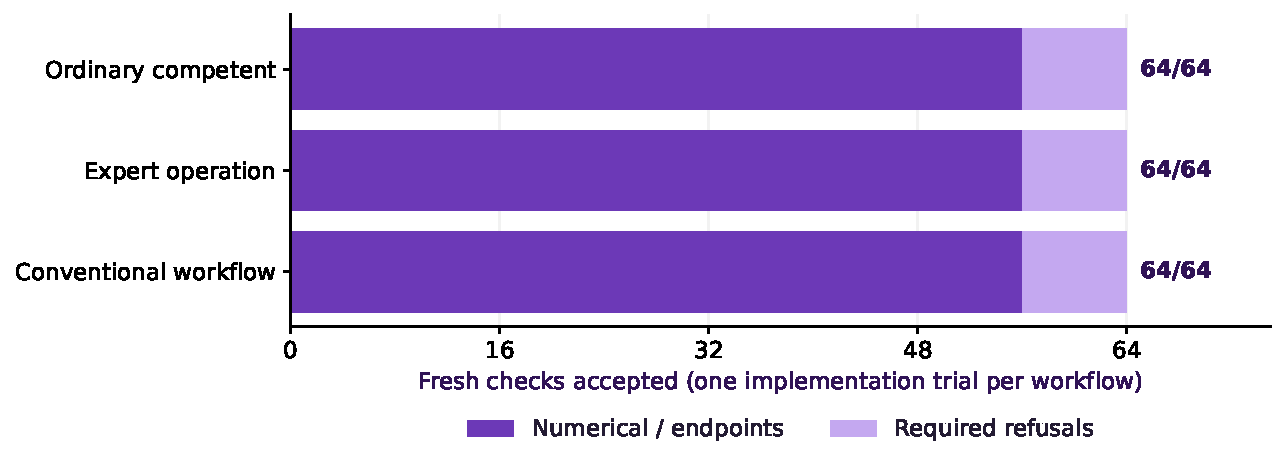
\includegraphics{figures/fresh_confirmation.pdf}
\caption{Primary fresh confirmation: all three frozen workflows satisfy
56 numerical or endpoint cases and eight refusals. The separately
disclosed known midpoint diagnostic is outside this denominator.}
\end{figure}

The independent root evaluator used 80- and 120-digit arithmetic, a
log-domain bisection inverse and a separately written incomplete-beta
continued fraction. It did not call Boost's inverse as its primary
judge. Analytic cases and exact rational integer-shape identities
provided additional controls. All 64 references were resolved. A
separate audit recomputed acceptance and used Decimal/Fraction controls;
its complete check record is supplied.

\hypertarget{what-the-checks-do-and-do-not-prove}{%
\subsection{What the checks do and do not
prove}\label{what-the-checks-do-and-do-not-prove}}

The bank establishes finite acceptance under a frozen contract. It does
not prove correctness throughout the continuous parameter envelope. Two
high-precision runs can share an error, and distinct programs can share
a mathematical ingredient. The evaluator therefore retains its
independent controls and uncertainty rather than treating agreement as a
proof of universal correctness.

Every primary call met its observed CPU limits: five seconds per call
and 120 seconds per worker. Raw timings are retained, but \textbf{no
numerical speedup is claimed}. Many recorded per-call CPU differences
were zero; the tiny batch and observed timer behavior do not support a
stable ratio. The identical reported peak memory high-water marks are
likewise unsuitable for an arm-level memory advantage. Import and build
time are recorded separately from solve time, and construction and
verification effort cannot be replaced by a microsecond solve-time
figure.

The broad result is uncomplicated: competent ordinary operation
succeeded, explicit expert operation succeeded, and the strongest
identified conventional workflow succeeded on the fresh bank. The expert
checklist did not produce a better primary accepted outcome in this
trial.

\hypertarget{the-additional-boundary-failure-stays-visible}{%
\subsection{The additional boundary failure stays
visible}\label{the-additional-boundary-failure-stays-visible}}

After primary confirmation, the independent audit ran an already-known
diagnostic at the smallest positive binary64 probability, with
\(a=1,b=2\). Ordinary and expert implementations returned the correct
positive subnormal value; the original conventional implementation
returned zero with \texttt{underflow}. This diagnostic was not fresh and
was not added to the primary denominator. A separately labeled
conventional correction, using ordinary analytic precision and lattice
rounding, passed the same 64-case replay plus the known midpoint
diagnostic. These are post hoc replays, not a new blind confirmation;
the original failure remains in the correction record. Neither the
original failure nor the corrected comparison disappears.

\editionbreak

\hypertarget{a-better-measuring-instrument}{%
\section{A better measuring
instrument}\label{a-better-measuring-instrument}}

The most instructive failure occurred in the numerical judge. Both the
ordinary and expert workstreams independently noticed that converting a
high-precision value to a machine float can conceal a subnormal rounding
error. Agreement at two precisions did not guarantee correct rounding.
The root evaluator initially shared that weakness.

The correction was made \textbf{before generating the fresh bank}. The
old evaluator, new evaluator, source hashes, diagnostic and rationale
remain in the package. The acceptance requirements did not change. All
three primary arms were evaluated by the same corrected instrument. We
disclose the feedback from the arm builders because the root evaluator
was not sealed from all development feedback.

\hypertarget{an-exact-counterexample}{%
\subsection{An exact counterexample}\label{an-exact-counterexample}}

Let \(\delta=2^{-1074}\), the smallest positive binary64 value. For a
Beta\((1,2)\) distribution,

\[
F(x)=2x-x^2.
\]

At the midpoint between zero and \(\delta\),

\[
F(\delta/2)=\delta-\delta^2/4<\delta.
\]

The quantile at probability \(\delta\) is therefore \textbf{above} that
midpoint and rounds to \(\delta\), not zero. A computation that loses
the tiny positive correction can land on the midpoint and apply the
wrong rounding decision. This is a numerical instrument failure with an
exact rational adjudication, not an invented new special function.

The corrected reference explicitly rounds on the binary64 subnormal
lattice. Near a midpoint, it uses an exact integer-shape CDF when
available, otherwise a 500-digit adaptive calculation with an
unresolved-reference outcome if the decision remains too close. The
construction uses conventional mathematical identities; the contribution
is the preserved diagnosis and the accountable correction.

\hypertarget{why-this-belongs-in-the-main-narrative}{%
\subsection{Why this belongs in the main
narrative}\label{why-this-belongs-in-the-main-narrative}}

A fluent implementation and a passing high-precision comparison can
still be wrong in the same way. A useful agent must be able to question
its checker and produce independently inspectable evidence for that
challenge. In this study, \textbf{ordinary competent use already did
that}. It would be misleading to award the behavior exclusively to the
expert arm.

Transformational Intelligence argues that evaluators may themselves
impose restrictions, but that revising an evaluator must not become a
way for a candidate to award itself victory. Its prescribed discipline
is an independent outcome anchor, preserved old evidence and a common
corrected comparison. This continuation exercises that discipline on a
real numerical instrument. It does not thereby establish a novel theory
of evaluator revision. (\protect\hyperlink{ref-ti}{Boucher 2026c})

The earlier kinetics construction remains supporting engineering. Its
conventional parity, thin conditional economics and untested physical
assumptions are unchanged. No chemical parameters, catalysts or
acceptance criteria were tuned in this continuation to manufacture a
second success.

\editionbreak

\hypertarget{the-commercial-offering-and-the-cost-boundary}{%
\section{The commercial offering and the cost
boundary}\label{the-commercial-offering-and-the-cost-boundary}}

The free delivered artifact is the recipient's strongest outside option.
A prospective paid engagement must therefore purchase \textbf{bounded
qualification, integration and handoff in one declared buyer
environment}, including correction and support. It cannot earn a license
premium for a public conventional algorithm. That buyer-specific
engagement has not been performed or accepted by a customer; the
following economics are conditional on it.

All amounts are nominal US dollars. Let \(M\) be the unknown additional
model/tool cost per future engagement, including retries and failed
attempts. Let \(D\) be the unknown complete historical cost of this
research, development and publication project. Neither is inferred from
wall time. The same \(M\) is used for all workflows because no metered
cost advantage was established. Historical \(D\) is deducted once for
full-project recovery, not again per customer.

\hypertarget{complete-central-cost-per-accepted-engagement}{%
\subsection{Complete central cost per accepted
engagement}\label{complete-central-cost-per-accepted-engagement}}

\begin{longtable}[]{@{}
  >{\raggedright\arraybackslash}p{(\columnwidth - 4\tabcolsep) * \real{0.3333}}
  >{\raggedright\arraybackslash}p{(\columnwidth - 4\tabcolsep) * \real{0.3333}}
  >{\raggedleft\arraybackslash}p{(\columnwidth - 4\tabcolsep) * \real{0.3333}}@{}}
\toprule\noalign{}
\begin{minipage}[b]{\linewidth}\raggedright
Item
\end{minipage} & \begin{minipage}[b]{\linewidth}\raggedright
Explicit central assumption
\end{minipage} & \begin{minipage}[b]{\linewidth}\raggedleft
Cost or receipt
\end{minipage} \\
\midrule\noalign{}
\endhead
\bottomrule\noalign{}
\endlastfoot
Net revenue & \$1,500 price, less 2\% expected refunds & \$1,470.00 \\
Successful delivery & 2.5 h at \$125/h: scope, integration,
qualification, handoff & \$312.50 \\
Failed attempts & 20\% failure probability; 1.5 h each; expected 0.375 h
per acceptance & \$46.875 \\
Support and correction & 0.5 h at \$125/h & \$62.50 \\
Acquisition & 0.75 h at \$125/h plus \$25 cash & \$118.75 \\
Infrastructure & Per accepted engagement & \$5.00 \\
Payment expense & Assumed 3\% of price plus \$0.30 & \$45.30 \\
Additional model/tools & All future engagement retries included &
\(M\) \\
\textbf{Contribution} & Before cohort fixed costs &
\textbf{\(879.075-M\)} \\
\end{longtable}

No recurring human review is invented for each automated scalar
calculation. These hours describe future buyer integration and service,
not observed labor in the present experiment. Loaded rates of
\$100--175/h are scoped estimates; historical employee wages provide
only an order-of-magnitude anchor, not contractor quotations. The
complete cost model discloses hours, rates and uncertainty.
(\protect\hyperlink{ref-bls}{US Bureau of Labor Statistics 2026})

Four central buyers share \$800 of maintenance and fixed business cost
over the cohort; \$500 of additional commercial setup is charged once.
That setup concerns service contracting and onboarding, not rebuilding
the already delivered code, tests or documentation. The central cohort
extends through day 115. The favorable cohort extends through day 195;
neither is an annual forecast.

\begin{longtable}[]{@{}llll@{}}
\toprule\noalign{}
Scenario & Buyers and price & Operating profit & Full-project return \\
\midrule\noalign{}
\endhead
\bottomrule\noalign{}
\endlastfoot
Favorable & 8 at \$2,500 & \(16,526.93-8M\) & \(16,226.93-8M-D\) \\
Central & 4 at \$1,500 & \textbf{\(2,716.30-4M\)} &
\textbf{\(2,216.30-4M-D\)} \\
Adverse & No buyers & \(-1,650\) & \(-3,050-D\) \\
\end{longtable}

\textbf{At an illustrative \(M=\$100\), central operating profit is
\$2,316.30; full-project return is \(1,816.30-D\).} This is a
sensitivity coordinate, not a measured model invoice. Operating profit
requires \(M<\$679.075\). At \(M=\$100\), the operating break-even price
is \$890.45; recovering additional setup raises it to \$1,022.03 before
historical \(D\). Full-project profitability remains unknown.

The adverse case preserves zero demand rather than forcing a sale. A
conditional-commitment gate can avoid its prospective setup and
fixed-cost loss. If an adverse low-price sale did occur, its unit
contribution would be negative even before model cost. Expected profit
is not an observed earning.

\editionbreak

\hypertarget{financing-demand-and-the-next-voluntary-exchange}{%
\section{Financing, demand and the next voluntary
exchange}\label{financing-demand-and-the-next-voluntary-exchange}}

\hypertarget{buyer-value-must-survive-the-free-alternative}{%
\subsection{Buyer value must survive the free
alternative}\label{buyer-value-must-survive-the-free-alternative}}

The central price hypothesis has little room for error. It assumes eight
hours of avoided self-qualification at \$150/h, \$600 of avoided delay,
and one hour of buyer participation. The resulting value ceiling is
\textbf{\$1,650}, leaving only \textbf{\$150 of modeled buyer surplus}
at the proposed \$1,500 fee. The hours and delay value are unmeasured. A
competent recipient needing only two hours to reuse the free artifact,
with no valuable delay avoided, may rationally buy nothing.

Prices are independent buyer hypotheses, not a fixed discount from an
invented market price. The executable sensitivity grid holds volume
fixed only to show arithmetic; it does not assume buyers remain when
price exceeds their value. Extra participation is not automatically
beneficial: replacing a \$125 provider hour with a \$150 buyer hour
increases combined cost unless it brings another justified benefit.

A human team attempting an equivalent new repair from the same public
recipe is estimated separately at 14--38 hours, or \$1,400--\$6,650 at
the stated rate endpoints. The central attempt estimate is 24 h at
\$125/h. This is neither a measured human baseline nor willingness to
pay, and it is never added as a second bill for the already produced
artifact.

\hypertarget{cash-comes-before-collection}{%
\subsection{Cash comes before
collection}\label{cash-comes-before-collection}}

At central \(M=\$100\), acquisition and pre-acceptance work precede
collection. The modeled peak expected cash deficit is
\textbf{\$2,091.25}. A separate \textbf{\$1,875 reserve} covers one
additional full refund and three extra correction hours. Required
unrestricted funding is therefore \textbf{\$3,966.25}. Actual available
funds, reserve balances, credit and financing commitments are unknown.
Any unpaid historical development obligation must be added.

An earned milestone can reduce the funding threshold to
\textbf{\$3,476.55}: 30\% is paid after a separately useful, accepted
qualification package; the remainder follows final accepted delivery.
This arrangement preserves the numerical requirements, refund exposure
and reserve. Two collection fees reduce central full-project return by
\$1.20 to \(1,815.10-D\) at the illustrative model-cost coordinate; the
initial calculation omitted that second fee and is preserved in the
economic correction record. It is a conditional contract design, not an
observed customer agreement or legal approval. A refundable deposit
stays restricted and supplies \textbf{zero unrestricted operating
capital}. A conditional commitment alone supplies no cash.

The reserve covers the specified stress, not multiple correlated
failures. Two extra full refunds exceed its refund component by \$1,500.
Delayed collection and financing fees can consume the margin. A reserve
is cash held, not an operating expense; it is not charged twice.

\hypertarget{sharing-is-available-to-the-conventional-team-too}{%
\subsection{Sharing is available to the conventional team
too}\label{sharing-is-available-to-the-conventional-team-too}}

\begin{longtable}[]{@{}
  >{\raggedright\arraybackslash}p{(\columnwidth - 2\tabcolsep) * \real{0.5000}}
  >{\raggedleft\arraybackslash}p{(\columnwidth - 2\tabcolsep) * \real{0.5000}}@{}}
\toprule\noalign{}
\begin{minipage}[b]{\linewidth}\raggedright
Matched arrangement, central \(M=\$100\)
\end{minipage} & \begin{minipage}[b]{\linewidth}\raggedleft
Return before historical \(D\)
\end{minipage} \\
\midrule\noalign{}
\endhead
\bottomrule\noalign{}
\endlastfoot
Conventional, four isolated engagements & \(-2,083.70\) \\
Expert operation alone, isolated & \(-2,083.70\) \\
Conventional, shared fixed costs & \(1,816.30\) \\
Expert operation plus shared fixed costs & \(1,816.30\) \\
\end{longtable}

This accounting counterfactual assumes equal capability and equal costs,
as the measured comparison warrants. The interaction attributable to
expert operation is zero. Sharing a known fixed cost can make a
conditional service viable; it is not a novel institution or exclusive
Alpha. All buyers retain the same public rights and can decline the
service.

\textbf{Observed commitments and collections: zero. Complete actual
project cost and available funds: unknown.} Buyer value, scope and costs
still need verification.

\editionbreak

\hypertarget{what-the-result-makes-possible}{%
\section{What the result makes
possible}\label{what-the-result-makes-possible}}

\hypertarget{evidence-a-small-capability-that-works-now}{%
\subsection{Evidence: a small capability that works
now}\label{evidence-a-small-capability-that-works-now}}

The demonstrated near-term capability is a bounded numerical incident
package: locate the relevant public evidence, reproduce the failure,
challenge the proposed novelty, construct a usable scalar component,
uncover a checker weakness, run fresh confirmation and deliver the
complete record. Its usefulness is inspectable without waiting for
physical fabrication, private data or a speculative future model.

The external libraries and public report do much of the intellectual
work. The live assistant's contribution is to connect them into an
executable, checked outcome under a time limit. That is a real
productive capability, even when a competent conventional team could
perform the same task. The study does not establish that the expert
operating procedure improves that capability over ordinary competent
use.

\hypertarget{conditional-expansion-a-portfolio-of-qualification-missions}{%
\subsection{Conditional expansion: a portfolio of qualification
missions}\label{conditional-expansion-a-portfolio-of-qualification-missions}}

A broader service could qualify numerical incidents across scientific
packages, supply bounded compatibility components and help recipients
decide whether to integrate, upgrade or decline a workaround. That
expansion depends on evidence absent from this single mission: multiple
prospectively selected incidents, real recipient acceptance, adequate
model metering, known licensing and support obligations, and a measured
rate of failures that cannot be repaired within the paid scope.

The next economically informative step is one voluntary buyer pilot with
a written acceptance contract and a capped integration scope. A valuable
customer question might be whether this component resolves a blocked
calculation on the buyer's actual supported stack. It must not be
silently replaced by passing our existing numerical bank. The free
artifact remains the buyer's outside option; a buyer who can
self-integrate cheaply has no reason to pay a premium merely because an
agent was involved.

\hypertarget{long-term-ambition-capabilities-that-open-better-opportunities}{%
\subsection{Long-term ambition: capabilities that open better
opportunities}\label{long-term-ambition-capabilities-that-open-better-opportunities}}

The flywheel's larger thesis is that a delivered capability can make a
later opportunity feasible. This result supplies a possible starting
asset, not evidence of compounding returns. A future successor could
reuse the source-pinning, numerical-regime analysis or exact-midpoint
checks on a genuinely new mission. It would still have to beat its own
competent baseline and an ordinary library containing the same asset
after retention, validation, integration and maintenance costs.

No fresh transfer trial was performed here. There is no retained-Alpha
or Gym-training claim. Adding transfer work would not repair the missing
expert advantage, and ordinary reuse is already available. Optional
learning investment should follow an expected benefit, not a prescribed
number of reinvestments.

Invent the Economy separates technical feasibility, participant value,
profitability, liquidity and actual exchange. Transformational
Autonomous Enterprises preserves comparisons in which a supplied
deterministic specialist matches quality and costs less. Those lessons
shape this edition: keep useful assets, let strong baselines win, and
require evidence for the next economic claim.
(\protect\hyperlink{ref-economy}{Boucher 2026a},
\protect\hyperlink{ref-tae}{2026b})

\textbf{Recommendation:} deliver the research artifact, retain the
corrected numerical instrument and conventional comparisons, and invite
a narrowly scoped customer qualification pilot. Stop the exclusive
algorithmic-novelty claim. Leave general Operational Alpha, discovery
advantage, retained benefit and realized commercial viability
unestablished until their own experiments support them.

\editionbreak

\hypertarget{reproducibility-provenance-and-publication}{%
\section{Reproducibility, provenance and
publication}\label{reproducibility-provenance-and-publication}}

\hypertarget{one-edition-several-readable-forms}{%
\subsection{One edition, several readable
forms}\label{one-edition-several-readable-forms}}

The package contains the compilable LaTeX manuscript, bibliography,
vector figures and plotting source; the polished PDF; a concise
executive brief; a complete offline HTML edition and a GitHub-readable
manuscript; frozen prompts, protocol, source and fresh results; the
conventional challenge and failures; the evaluator correction;
independent audit; executable economics; and a LinkedIn draft that has
not been posted.

The Markdown manuscript is the common content source for the LaTeX and
HTML editions. Numerical facts are checked against the machine-readable
result and economic files. The brief repeats the same verdicts and
conditions. Download identities and the publication status are recorded
separately so a review upload cannot be confused with a canonical
release.

The deterministic reproduction entry point rebuilds kernels in isolated
copies, replays the frozen case bank, recomputes references and scores,
and preserves the original source hashes. The native bridge reuses the
existing Journal, CostLedger and fitness components; it does not build a
second registry or invent a customer payment. Unknown actual charges
remain unknown. Its local research identity is not a live external
authentication claim.

\hypertarget{evidence-and-source-identities}{%
\subsection{Evidence and source
identities}\label{evidence-and-source-identities}}

\begin{longtable}[]{@{}
  >{\raggedright\arraybackslash}p{(\columnwidth - 2\tabcolsep) * \real{0.5000}}
  >{\raggedright\arraybackslash}p{(\columnwidth - 2\tabcolsep) * \real{0.5000}}@{}}
\toprule\noalign{}
\begin{minipage}[b]{\linewidth}\raggedright
Item
\end{minipage} & \begin{minipage}[b]{\linewidth}\raggedright
Identity or location
\end{minipage} \\
\midrule\noalign{}
\endhead
\bottomrule\noalign{}
\endlastfoot
Edition & \texttt{DIGITAL-20261027-R1} \\
Repository audit source &
\texttt{3947e4ec8fd74ad40e13e8ff825a149fa98a10e9} \\
Boost.Math construction source &
\texttt{70a36632cfbfe6a862cd8a5b88b357ca3a770a3d} \\
SciPy inspected source &
\texttt{37fad094584e1129ea652680608cd2c1b02463b9} \\
Acceptance protocol & \texttt{experiment/protocol.json} and SHA-256
sidecar \\
Fresh source and case freeze & \texttt{experiment/source\_freeze.json},
\texttt{fresh\_case\_metadata.json} \\
Primary result & \texttt{experiment/comparison\_results.json} \\
Instrument correction &
\texttt{experiment/evaluator\_correction.json} \\
Complete claim map & \texttt{delivery/claim\_map.json} \\
Monetary model & \texttt{economics/economics.py} and scenario outputs \\
\end{longtable}

All 24 preserved upstream component files were verified identical at the
prior and current repository snapshots. Third-party licenses remain
attached to their sources. Frozen experimental originals are retained
byte for byte; any publication-normalized or corrected copies have
separate identities. The previous gap archive is preserved with its
original SHA-256 in the continuation provenance.

\hypertarget{publication-is-a-separate-acceptance-boundary}{%
\subsection{Publication is a separate acceptance
boundary}\label{publication-is-a-separate-acceptance-boundary}}

The authorized route is an additive study review branch and draft pull
request under \texttt{studies/agi-alpha-digital-outcome-20261027-2206/}.
The mixed source, data and HTML package takes the repository's full
review lane. It is not a passive-paper exemption. Existing runtime,
discovery, accounting and publication owners retain their roles.
(\protect\hyperlink{ref-coordination}{MONTREAL.AI 2026a},
\protect\hyperlink{ref-publication}{2026b})

This edition may be inspected and downloaded from its pinned review
source. Canonical production publication requires the existing owner's
exact-source review, required hosted checks, qualified integration and
actual public deployment/served-byte verification. A green preparation
workflow with skipped deployment does not establish publication. The
delivery receipt states the exact source, public reading page, downloads
and any remaining external dependency; it does not borrow a prior
release's approval.

\clearpage

\hypertarget{appendix-preserved-failures-and-claim-boundaries}{%
\section{Appendix: preserved failures and claim
boundaries}\label{appendix-preserved-failures-and-claim-boundaries}}

\hypertarget{corrections-without-erasure}{%
\subsection{Corrections without
erasure}\label{corrections-without-erasure}}

\begin{longtable}[]{@{}
  >{\raggedright\arraybackslash}p{(\columnwidth - 4\tabcolsep) * \real{0.3333}}
  >{\raggedright\arraybackslash}p{(\columnwidth - 4\tabcolsep) * \real{0.3333}}
  >{\raggedright\arraybackslash}p{(\columnwidth - 4\tabcolsep) * \real{0.3333}}@{}}
\toprule\noalign{}
\begin{minipage}[b]{\linewidth}\raggedright
Record
\end{minipage} & \begin{minipage}[b]{\linewidth}\raggedright
Observed problem
\end{minipage} & \begin{minipage}[b]{\linewidth}\raggedright
Treatment
\end{minipage} \\
\midrule\noalign{}
\endhead
\bottomrule\noalign{}
\endlastfoot
Early Boost challenge & One long-double configuration failed a public
example & Preserved beside the successful double configuration; no
weak-only baseline \\
Ordinary development & Subnormal rounding and an unscaled quadrature
oracle produced misleading evidence & Original attempts retained;
lattice rounding and normalized controls added before freeze \\
Expert development & Wrong finite subnormal-tail outputs and
high-precision conversion error & Trigger and rounding repairs made
before freeze; original attempts retained \\
Root evaluator v1 & Direct high-precision-to-float conversion could
double-round & v1 retained; exact midpoint controls and v2 freeze before
fresh generation \\
Conventional primary source & Known post-confirmation Beta\((1,2)\)
midpoint returned underflow & Failure retained outside primary
denominator; correction separately labeled \\
Expert packaging & Storage exhaustion interrupted README creation &
Partial attempt and recovery recorded; no numerical source erasure \\
Root freeze check & A hash copied into a summary contained a
transcription error & Original source manifest rechecked; no source
mutation or case generation occurred before resolution \\
\end{longtable}

\hypertarget{what-each-positive-result-can-support}{%
\subsection{What each positive result can
support}\label{what-each-positive-result-can-support}}

\begin{itemize}
\tightlist
\item
  \textbf{Runnable construction:} yes, within the stated scalar envelope
  and finite tested cases. It is not universal proof or upstream
  integration.
\item
  \textbf{Fresh research acceptance:} 64/64 checks for each original
  frozen arm, under a common corrected evaluator. Known diagnostic
  limitations remain visible.
\item
  \textbf{Commercial operating profit:} conditional model only, with
  price, volume, scope, failure, support and unknown model-cost
  thresholds. No observed sale.
\item
  \textbf{Financing feasibility:} conditional on actual unrestricted
  funds or explicitly agreed stages. Refundable balances do not become
  operating capital.
\item
  \textbf{Operational Alpha:} not established. The expert arm did not
  improve primary accepted quality over competent ordinary use; complete
  cost and broad replication are missing.
\item
  \textbf{Transformational contribution:} no exclusive numerical
  advance. Established methods meet the useful outcome; the public
  reporter supplied the formulation.
\item
  \textbf{Fresh-transfer benefit:} untested. Ordinary reusable-library
  access remains a required comparator for a future transfer study.
\end{itemize}

\hypertarget{research-limits-that-affect-the-headline}{%
\subsection{Research limits that affect the
headline}\label{research-limits-that-affect-the-headline}}

One implementation trial per arm on one public mission cannot establish
population performance. Provider identity, billing and buyer demand are
unmeasured. Independent implementation and audit occurred within one
coordinated assistant session. Finite scalar acceptance does not justify
broader product claims. The conventional midpoint defect and post hoc
correction stay outside fresh confirmation. Human-service estimates are
assumptions, not quotations or willingness to pay.

\clearpage

\hypertarget{references}{%
\section{References}\label{references}}

\hypertarget{refs}{}
\begin{CSLReferences}{1}{0}
\leavevmode\vadjust pre{\hypertarget{ref-boost}{}}%
Boost.Math Developers. 2026. {``The Incomplete Beta Function
Inverses.''}
\url{https://www.boost.org/doc/libs/latest/libs/math/doc/html/math_toolkit/sf_beta/ibeta_inv_function.html}.

\leavevmode\vadjust pre{\hypertarget{ref-economy}{}}%
Boucher, Vincent. 2026a. {``Invent the Economy.''}
\url{https://github.com/MontrealAI/AGI-Alpha-Agent-v0/blob/3947e4ec8fd74ad40e13e8ff825a149fa98a10e9/docs/Invent_the_Economy.tex}.

\leavevmode\vadjust pre{\hypertarget{ref-tae}{}}%
---------. 2026b. {``Transformational Autonomous Enterprises.''}
\url{https://github.com/MontrealAI/AGI-Alpha-Agent-v0/blob/3947e4ec8fd74ad40e13e8ff825a149fa98a10e9/docs/papers/transformational-autonomous-enterprises-v1.tex}.

\leavevmode\vadjust pre{\hypertarget{ref-ti}{}}%
---------. 2026c. {``Transformational Intelligence: Learning to Change
the Game.''}
\url{https://github.com/MontrealAI/AGI-Alpha-Agent-v0/blob/3947e4ec8fd74ad40e13e8ff825a149fa98a10e9/docs/Transformational_Intelligence.tex}.

\leavevmode\vadjust pre{\hypertarget{ref-scipyissue}{}}%
chrisb83. 2026. {``{BUG}: Beta Quantile Failures in Extreme Tails, Issue
26531.''} \url{https://github.com/scipy/scipy/issues/26531}.

\leavevmode\vadjust pre{\hypertarget{ref-coordination}{}}%
MONTREAL.AI. 2026a. {``AGI ALPHA Coordination Record, Issue 4850.''}
\url{https://github.com/MontrealAI/AGI-Alpha-Agent-v0/issues/4850}.

\leavevmode\vadjust pre{\hypertarget{ref-publication}{}}%
---------. 2026b. {``Research Paper Upload and Publication Policy.''}
\url{https://github.com/MontrealAI/AGI-Alpha-Agent-v0/blob/3947e4ec8fd74ad40e13e8ff825a149fa98a10e9/docs/agent/PAPER_UPLOADS.md}.

\leavevmode\vadjust pre{\hypertarget{ref-dlmf}{}}%
National Institute of Standards and Technology. 2026. {``Digital Library
of Mathematical Functions, Section 8.17: Incomplete Beta Functions.''}
\url{https://dlmf.nist.gov/8.17}.

\leavevmode\vadjust pre{\hypertarget{ref-scipydocs}{}}%
SciPy Developers. 2026. {``Scipy.special.betaincinv.''}
\url{https://docs.scipy.org/doc/scipy/reference/generated/scipy.special.betaincinv.html}.

\leavevmode\vadjust pre{\hypertarget{ref-statsmodels}{}}%
statsmodels contributors. 2026. {``Boundary Confidence Interval Issues
and Active Repairs.''}
\url{https://github.com/statsmodels/statsmodels/issues/10536}.

\leavevmode\vadjust pre{\hypertarget{ref-sympy}{}}%
SymPy contributors. 2026. {``Kronecker Product Public Report and
Existing Repair.''} \url{https://github.com/sympy/sympy/issues/30860}.

\leavevmode\vadjust pre{\hypertarget{ref-bls}{}}%
US Bureau of Labor Statistics. 2026. {``Software Developers, Quality
Assurance Analysts, and Testers.''}
\url{https://www.bls.gov/ooh/computer-and-information-technology/software-developers.htm}.

\end{CSLReferences}

\end{document}
